\chapter{\label{sec:square_root}Grazing és square-root mapping}

\exampleheading{Motiváló példa: a rezgő test eléri az ütközőt.}
Gondoljunk egy rugón rezgő tömegre, amelynek mozgását egy merev ütköző korlátozza. Kis gerjesztésnél a test nem ér a falhoz; a gerjesztés növelésekor a pálya először éppen érinti azt, nulla normálsebességgel. Ez a \emph{grazing}, azaz nulla normálsebességű érintkezés. Kissé nagyobb kitérésnél már ütközés következik be. Hogyan függ az ütközés hatása a határtól való kis eltéréstől?

Legyen $h(t)$ a faltól mért előjeles távolság, a megengedett oldalon $h>0$. Az ütközést egyelőre figyelmen kívül hagyva, a pálya minimuma közelében legyen
\begin{equation}\label{eq:grazing_motivation}
h(t)\simeq-\varepsilon+\frac{a}{2}(t-t_g)^2,\qquad a>0.
\end{equation}
\begin{figure}[htbp]\centering
% Local quadratic geometry, illustrated for epsilon>0; 11 pt labels.
\begin{tikzpicture}[x=2.3cm,y=1.1cm,>=Latex,line width=.7pt,
 font=\normalfont\fontsize{11}{13.2}\selectfont]
\fill[gray!10] (-2.05,-1.4) rectangle (2.05,0);
\draw[->] (-2.1,0)--(2.3,0) node[right] {$t$};
\draw[->] (-2,-1.4)--(-2,3.2) node[above] {$h(t)$};
\node[above right] at (1.2,0) {$h=0$: fal};
\node[above right] at (-1.85,2.8) {megengedett oldal: $h>0$};
\draw[blue!65!black,very thick,domain=-1.9:-1,samples=50]
 plot (\x,{\x*\x-1});
\draw[blue!65!black,thick,dashed,domain=-1:1.9,samples=100]
 plot (\x,{\x*\x-1});
\draw[densely dotted] (0,-1.25)--(0,2.7);
\fill (-1,0) circle (1.5pt); \fill (0,-1) circle (1.5pt);
\draw (1,-.06)--(1,.06);
\node[above left,fill=white,inner sep=1pt] at (-1,0) {$t_-$};
\node[above left] at (0,0) {$t_g$};
\node[below right] at (1,0) {$t_+$};
\draw[<->] (.12,0)--(.12,-1) node[midway,right] {$\varepsilon$};
\node[below] at (0,-1.06) {$h(t_g)=-\varepsilon$};
\draw[densely dotted] (-1,-.12)--(-1,-1.85);
\draw[densely dotted] (0,-1.45)--(0,-1.85);
\draw[<->] (-1,-1.75)--(0,-1.75)
 node[midway,below] {$t_g-t_-=\sqrt{2\varepsilon/a}$};
\node[align=center] at (0,-2.8) {szaggatott: ütközés nélküli\\sima továbbvezetés};
\end{tikzpicture}

\caption{A \eqref{eq:grazing_motivation} lokális parabolaközelítés geometriai jelentése, $\varepsilon>0$ esetén. A folytonos ág a beérkező mozgás; a szaggatott görbe az ütközést figyelmen kívül hagyó folytatás. A szürke tartomány a merev fal esetén nem megengedett.}\label{fig:grazing_parabola}
\end{figure}
A \ref{fig:grazing_parabola}. ábrán a függőleges tengely az előjeles faltávolság, a vízszintes az idő. A parabola minimuma $(t_g,-\varepsilon)$; az $a>0$ a görbületet meghatározó normálgyorsulás. A falat először a bal oldali $t_-$ gyöknél érjük el. A $h=0$ feltételből $(t-t_g)^2=2\varepsilon/a$, ezért az érintési időhöz viszonyított eltérés négyzetgyökösen függ $\varepsilon$-tól. A jobb oldali $t_+=t_g+\sqrt{2\varepsilon/a}$ csak a simán továbbvezetett parabola második gyöke: a tényleges ütköző pálya már $t_-$-nál visszapattan, és onnantól más görbét követ. Ha $\varepsilon=0$, a parabola éppen érinti a falat; $\varepsilon<0$ esetén a minimum is felette marad.

Itt $t_g$ a minimum időpontja, $a$ a helyi normálgyorsulás, $\varepsilon$ pedig az ütközés nélküli pálya legnagyobb behatolása. Ez utóbbi csak a simán továbbvezetett pálya geometriai jellemzője: a merev falon a tényleges pálya nem halad át. Ha $\varepsilon<0$, nincs ütközés; $\varepsilon=0$ a grazing; $\varepsilon>0$ esetén a beérkező ág első falelérése és sebessége vezető rendben
\begin{equation}\label{eq:grazing_motivation_speed}
t_-=t_g-\sqrt{\frac{2\varepsilon}{a}},\qquad
v^-\simeq-\sqrt{2a\varepsilon}.
\end{equation}
A $v^+=-rv^-$ visszapattanási törvény ezért
\begin{equation}\label{eq:grazing_motivation_jump}
\Delta v=v^+-v^-\simeq(1+r)\sqrt{2a\varepsilon}
\end{equation}
sebességugrást eredményez. Például $a=1\,\mathrm{m/s^2}$ és $r=0{,}8$ mellett $\varepsilon=0{,}01\,\mathrm{mm}$ esetén $\Delta v\simeq0{,}00805\,\mathrm{m/s}$; százszor nagyobb behatolás tízszer nagyobb sebességugrást ad. A kapcsolat tehát négyzetgyökös, nem lineáris.

Ha az ütközés utáni mozgást egy rögzített metszetig továbbvezetjük, ez a kis sebességváltozás a visszatérési állapotban is általában $\sqrt{\varepsilon}$ rendű korrekciót okoz. Innen ered a \emph{square-root mapping}. Az együttható és az irány a további mozgástól és a metszettől függ; a fenti helyi számítás még nem a teljes visszatérési leképezés. A korrekció nullához tart, de érzékenysége $\varepsilon\to0^+$ esetén korlátlanná válhat. Ez magyarázza, miért romlik el a szokásos lineáris közelítés a grazing közelében.

Ilyen geometria jelenhet meg hézagos mechanizmusok, ütközővel határolt rezgések vagy egy akadályt éppen elérő periodikus pálya esetén. A következő ütköző oszcillátor ezt a helyzetet modellezi. A levezetés nemelfajuló, merev ütközésre vonatkozik; tartós kontaktushoz vagy $a=0$ érintkezéshez más helyi modell szükséges.


Tekintsük az alábbi rendszert:
\begin{equation}
\dot{x}=F(x), \quad \text{ahol } x\in S^+=\left\{x\in\mathcal{D}\subset\mathbb{R}^n: H(x)>0\right\},
\end{equation}
amely a
\begin{equation}
\Sigma:=\left\{x\in\mathcal{D}: H(x)=0\right\}
\end{equation}
felületen ütközik az
\begin{equation}
x^+=R(x^-):=x^-+W(x^-)v_H(x^-)
\end{equation}
leképezés által kijelölt módon. $H(x)$ a kapcsolóvonal egyenlete, $x^+$ az ütközés utáni állapotváltozó, $x^-$ pedig az ütközés előtti állapotváltozó. Az ütközés pillanatában a kapcsolófelületre merőleges sebességet és gyorsulást a
\begin{equation}
v_H(x)=H_xF(x),
\end{equation}
a gyorsulást pedig
\begin{equation}
 a_H(x)=F(x)^\mathsf T H_{xx}(x)F(x)+H_x(x)F_x(x)F(x)
\end{equation}
összefüggésekkel adjuk meg. Ezek $H$ első és második időderiváltjai; geometriai normálsebességgel csak megfelelően normalizált $H$ esetén azonosak. A $H_{xx}$ Hess-mátrix. A továbbiakban $a_H$-t röviden $a$ jelöli.
\exampleend

\section{1DoF ütköző oszcillátor}
\examplebody

Az ütköző oszcillátor alapmodelljéhez és periodikus mozgásához lásd \cite[1.2.1--1.2.2. és 6.1. szakasz]{dib}.


Az 1 DoF ütköző oszcillátor dimenziótlan egyenlete az alábbi:
\begin{equation}
u''(t)+2\zeta u'(t)+u(t)=w(t),\qquad u(t)>\sigma,\qquad \zeta\geq0.
\end{equation}
A $t=t_0$ (ütközéskori) időpillanatban az alábbi leképezés valósul meg:
\begin{equation}
f(u^-,v^-):=(u^+,v^+),
\end{equation}
ahol közvetlenül az ütközés előtti pozíció és sebesség
\begin{equation}
u^-=u(t_0),
\end{equation}
\begin{equation}
v^-=v(t_0)=\left.\frac{\mathrm{d}u}{\mathrm{d}t}\right|_{t=t_0},
\end{equation}
továbbá a közvetlenül az ütközés utáni pozíció és sebesség felírható az alábbi módon:
\begin{equation}
u^+=u^-,
\end{equation}
\begin{equation}
v^+=-rv^-, \quad 0\le r\le 1.
\end{equation}
Megjegyzés: $1-r^2$ meghatározza az ütközés során elnyelt mozgási energiaarányt. $r$ a különböző anyagok tulajdonságaitól függ, $r$ értékét mérésből vagy kontaktusmodellből kell meghatározni; az ábrákon $r=0{,}95$ egy választott példa. $r=1$ a tökéletesen rugalmas és $r=0$ a tökéletesen rugalmatlan ütközésnek felel meg. Az általunk vizsgált esetben $w(t)=\cos(\omega t)$ a periodikus gerjesztés $\frac{2\pi}{\omega}$ periódussal:
\begin{equation}
u''(t)+2\zeta u'(t)+u(t)=\cos(\omega t),\qquad u>\sigma.
\end{equation}
Az 1DoF ütköző oszcillátor átírható az alábbi három-dimenziós autonóm rendszerré:
\begin{equation}
\begin{split}
\frac{\mathrm{d}u}{\mathrm{d}t}&=v,\\
\frac{\mathrm{d}v}{\mathrm{d}t}&=-u-2\zeta v+w(s),\\
\frac{\mathrm{d}s}{\mathrm{d}t}&=1,
\end{split}\qquad \qquad \text{ha } u>\sigma,
\end{equation}
azaz az alábbi autonóm rendszer adódik. A $w(s)=\cos(\omega s)$ miatt a kibővített rendszer nem lineáris:
\begin{equation}
\dot{x}=F(x),
\end{equation}
ahol
\begin{equation}\label{eq:xFx}
x=\begin{pmatrix}
u\\ v\\ s
\end{pmatrix},\qquad
F(x)=\begin{pmatrix}
v\\
-u-2\zeta v+w(s)\\
1
\end{pmatrix}.
\end{equation}
A kapcsolóvonal egyenlete
\begin{equation}
H(x)=u-\sigma,
\end{equation}
gradiense pedig

\begin{equation}\label{eq:hx}
H_x=\begin{pmatrix}1&0&0\end{pmatrix}.
\end{equation}
A leképezés a kapcsolóvonalon:

\begin{equation}
x \rightarrow R(x)=\begin{pmatrix}
u\\
-r v\\
s,
\end{pmatrix}
\end{equation}
azaz a reset leképezés Jacobi-mátrixa

\begin{equation}\label{eq:Rx}
R_x(x)=\begin{pmatrix}
1 & 0 & 0\\
0 & -r & 0\\
0 & 0 & 1
\end{pmatrix}.
\end{equation}
A sebesség, illetve a gyorsulás az alábbi módon írható le:
\begin{equation}
v_H(x)=v,
\end{equation}
\begin{equation}
a(x)=-u-2\zeta v+w(s),
\end{equation}
így kapcsolóvonalra történő becsapódási sebesség:

\begin{equation}
H_x(x^-) F(x^-) = v^-,
\end{equation}
Újra megemlítjük a \eqref{eq:Qxmatrix} egyenletre levezetett korrekciós mátrixot:

\begin{equation}\label{eq:Qxmatrix2}
Q_x(x^-)=R_x(x^-)+\frac{F(R(x^-))-R_x(x^-)F(x^-)}{H_x(x^-)F(x^-)}H_x(x^-)\,,
\end{equation}
ahol $x^-$ legyen egy periodikus pálya ütközési pontja. Felhasználva, hogy
\begin{equation}
x^+=R(x^-),
\end{equation}
azaz az ütközés utáni állapot felírható az ütközés előtti állapot és leképezés segítségével. \eqref{eq:xFx}, \eqref{eq:hx}, \eqref{eq:Rx} egyenletek felhasználásával:

\begin{equation}
\begin{split}
Q_x(x^-)=\begin{pmatrix}
1 & 0 & 0\\
0 & -r & 0\\
0 & 0 & 1
\end{pmatrix}+\frac{\left(F(x^+)-R_x(x^-)F(x^-)\right)H_x}{v^-}=\\
=\begin{pmatrix}
1 & 0 & 0\\
0 & -r & 0\\
0 & 0 & 1
\end{pmatrix}+\frac{1}{v^-}\left(\begin{pmatrix}
v^+-v^-\\
a^++ra^-\\
1-1
\end{pmatrix} \right)H_x=\begin{pmatrix}
-r & 0 & 0\\
\frac{a^++ra^-}{v^-} & -r & 0\\
0 & 0 & 1
\end{pmatrix}.
\end{split}
\end{equation}

A \ref{fig:phase}--\ref{fig:ut}. ábrák ugyanannak a három numerikus megoldásnak két nézetét mutatják. Mindhárom esetben $\sigma=0$, $r=0{,}95$, $\zeta=0$, a kezdeti állapot $u(0)=1$, $v(0)=0$, a gerjesztés pedig $\cos(\omega t)$. A frekvenciák rendre $\omega=3$, $2{,}76$ és $2{,}9$. A $T=2\pi/\omega$ gerjesztési periódussal mérve $100T$ ideig számoltunk, és az utolsó tizenkét periódust, a $[88T,100T]$ ablakot ábrázoljuk. Az elhagyott kezdeti szakasz csökkenti a kezdeti feltétel hatását; ez önmagában nem bizonyítja, hogy a megmaradó mozgás periodikus vagy már teljesen állandósult.

A szabad mozgás szakaszai a csillapítatlan egyenlet pontos megoldásából származnak; az $u=0$ eseményidőket gyökkereséssel határoztuk meg, majd a $v^+=-rv^-$ reset leképezést alkalmaztuk. A reprodukálható ábragenerátor a \texttt{codes/impact\_figures\_v3.py}; a rövid MATLAB-példa a \texttt{codes/impact\_portraits\_v3.m}, amely az \ref{ap:codes1}. függelék eseményvezérelt integrátorát használja.

\begin{figure}[p]
\centering
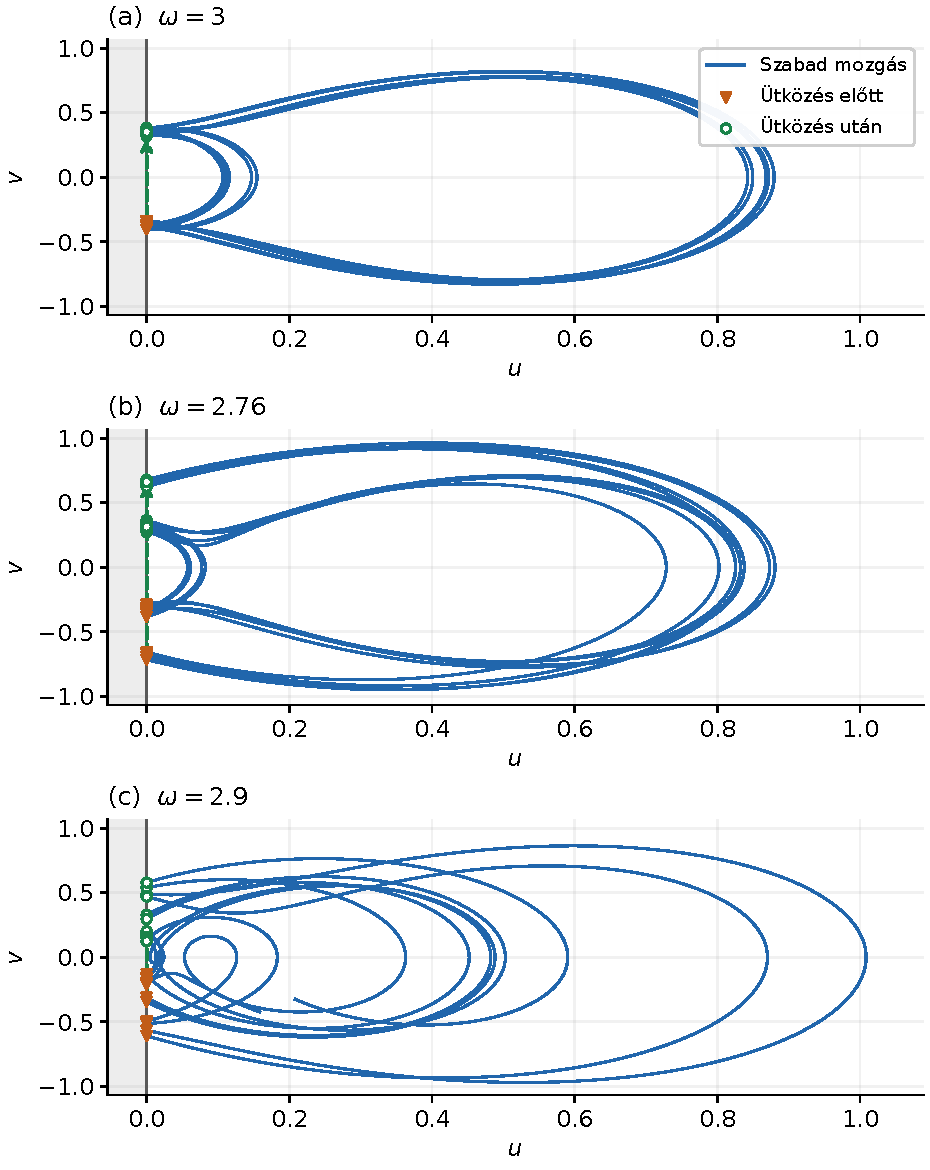
\includegraphics[width=.95\linewidth]{graphics_v3/impact_phase.pdf}
\caption{Az ütköző oszcillátor $(u,v)$ fázissíkbeli vetülete három frekvencián, azonos tengelyskálákkal. Kék: szabad mozgás; narancssárga háromszög: ütközés előtti állapot; zöld üres kör: ütközés utáni állapot. A fal $u=0$, a szürke oldal nem megengedett. Panelenként egy szaggatott nyíl szemlélteti a sebességugrást.}\label{fig:phase}
\end{figure}


A \ref{fig:phase}. ábrán a vízszintes koordináta az elmozdulás, a függőleges a sebesség. A $v<0$ ágakon a tömeg a fal felé halad, a $v>0$ ágakon távolodik tőle; a $v=0$, $u>0$ pontok a kitérés fordulópontjai. A falat a pálya $(0,v^-)$ pontban éri el, majd ugyanazon helyen $(0,-rv^-)$ állapotból folytatódik. Az ezt összekötő szaggatott nyíl pillanatszerű állapotugrást jelöl, nem a szabad mozgás egy szakaszát. A kisebb visszapattanási sebesség miatt az ütközés utáni jel közelebb van a $v=0$ tengelyhez, mint a hozzá tartozó beérkező jel.

Az ismételten bejárt ívek egymásra rajzolódhatnak, ezért egyetlen látható ív több időbeli bejárást is takarhat. A különböző falelérési sebességek eltérő ütközési állapotokat jeleznek. Fontos, hogy ez a háromdimenziós $(u,v,s)$ rendszer kétdimenziós vetülete: azonos $(u,v)$ ponton különböző gerjesztési fázisokban is áthaladhat a megoldás. A vetületi kereszteződés ezért nem sérti a megoldás egyértelműségét. A bonyolultabb vonalrajz önmagában nem bizonyít káoszt; ehhez például Poincaré-metszetet vagy Ljapunov-exponenst kell vizsgálni.

\begin{figure}[p]
\centering
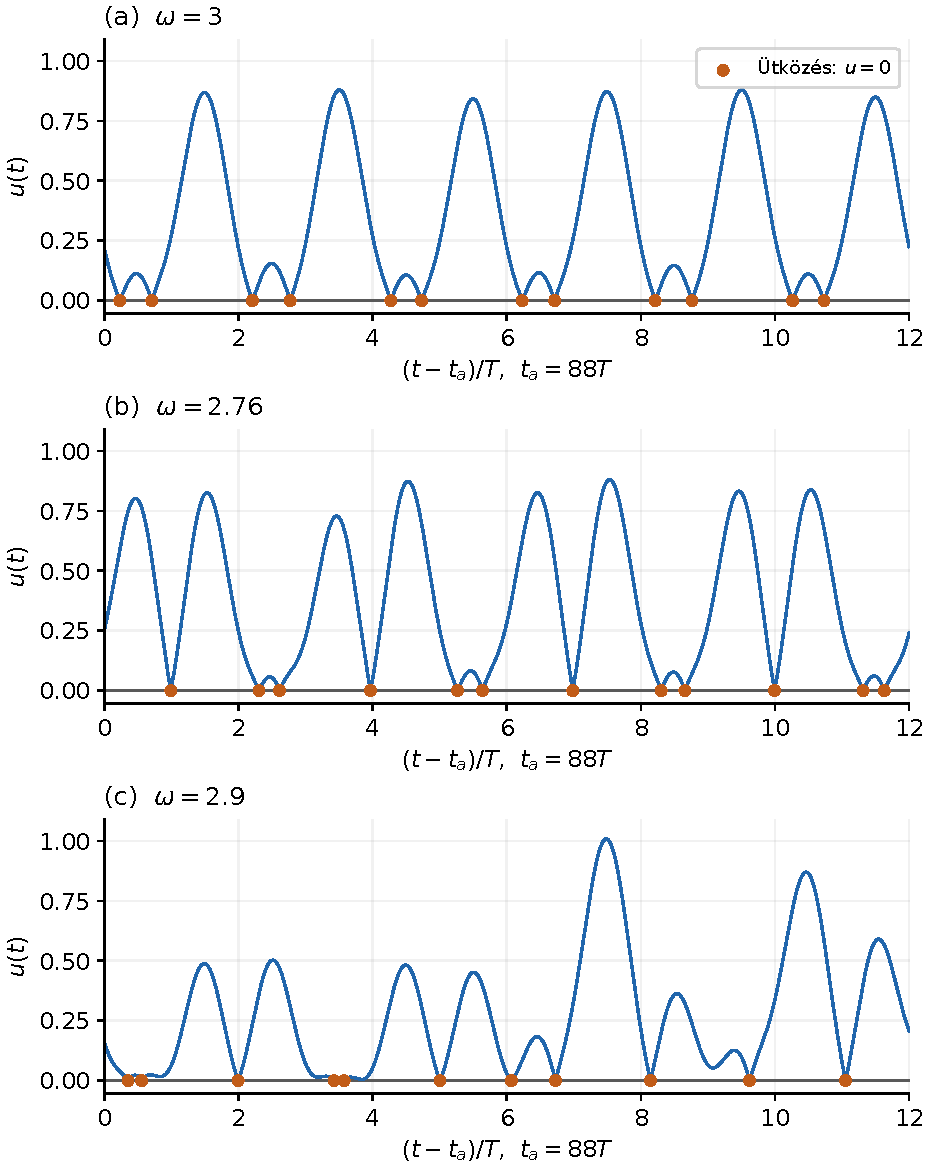
\includegraphics[width=.95\linewidth]{graphics_v3/impact_time.pdf}
\caption{A \ref{fig:phase}. ábra pályái az időtartományban, azonos elmozdulásskálával. A vízszintes tengely a $t_a=88T$ időponttól eltelt gerjesztési periódusok száma. A narancssárga pontok az ütközéseket jelölik; a folytonos elmozdulásgörbe meredeksége ekkor ugrik.}\label{fig:ut}
\end{figure}


A \ref{fig:ut}. ábra megmutatja az ütközések sorrendjét és a köztük eltelt időt, amit a fázisábrán az egymásra rajzolódó ívek elfedhetnek. Minden narancssárga pontban $u=0$, de a test nem halad a fal mögé. A kitérés folytonos marad, miközben a bal oldali meredekség $v^-<0$ értékről a jobb oldali $v^+=-rv^->0$ értékre ugrik: ezért látható csúcsos minimum az ütközésnél. A falhoz csak kis sebességgel érkező pályának kisebb a meredekségugrása; a grazing határesetben $v^-=0$ és az érintés simává válhat.

A megjelenített ablakban az (a) panelen közel ismétlődő nagy és kis kitérések váltakoznak; a (b) panelen a nagy kitérések közé kis, fal közeli visszapattanások ékelődnek; a (c) panelen a csúcsmagasságok és az ütközési időközök változatosabbak. Ezek a választott véges időablak megfigyelései, nem a mozgások bizonyított dinamikai osztályozása. A hosszú idejű részletes ütközéssor érzékeny lehet a numerikus kerekítésre; a két ábra ugyanazon számítás adatait használja.

A panelek összevetésével a csúcskitérések és az ütközések közti idő változását lehet leolvasni. Egy vízszintes egység minden panelben egy gerjesztési periódus, de eltérő $\omega$ mellett eltérő fizikai időt jelent. A $\zeta=0$ választás csak a folytonos viszkózus csillapítást kapcsolja ki: az $r<1$ ütközési törvény továbbra is energiát veszít, amelyet a gerjesztés részben pótolhat.

A mátrixok a \emph{perturbációkat}, nem magukat az állapotokat képezik le. Ha a periódus egy folytonos szakasszal és annak végén egy ütközéssel írható le, akkor
\[
\delta x^- = M\delta x_0,\qquad
\delta x^+ = Q_x\delta x^-,\qquad
\mathcal M=Q_xM.
\]
Általában a folytonos szakaszok variációs mátrixait és az események korrekciós mátrixait időrendi sorrendben kell összeszorozni; az időben későbbi tényező balra kerül. A $3\times3$ autonóm leírásból rögzített gerjesztési fázisnál a $2\times2$ állapotérzékenységet használjuk. A továbbiakban az ütközési képletben $Q_x$ ezt a kétdimenziós blokkot jelenti.
\exampleend

\section{Ütközés nélküli eset -- monodrómia-mátrix}
Tegyük fel, hogy $\left(u(t),v(t)=\frac{\mathrm{d}u}{\mathrm{d}t}\right)$ megoldása a
\begin{equation}
u''(t)+2\zeta u'(t)+u=w(t)
\end{equation}
egyenletnek. Tekintsük az alábbi perturbált megoldást: $\left(u(t)+\delta u(t),v(t)+\delta v(t)\right)$. A $\delta u$ függvény kielégíti az alábbi variációs egyenletet
\begin{equation}
\delta u''(t)+2\zeta \delta u'(t)+\delta u=0,\qquad \left(\delta u(t_0),\delta v(t_0) \right)=\left(\delta u_0,\delta v_0 \right),
\end{equation}
azaz
\begin{equation}
\frac{\mathrm{d}}{\mathrm{d}t}\begin{pmatrix}
\delta u\\ \delta v
\end{pmatrix}=L\begin{pmatrix}
\delta u\\ \delta v
\end{pmatrix}:=\begin{pmatrix}
0 & 1 \\
-1 & -2\zeta
\end{pmatrix}\begin{pmatrix}
\delta u\\ \delta v
\end{pmatrix}.
\end{equation}
Így felírható az egy $(T)$ periódusra vonatkozó állapotvektor variációja:
\begin{equation}
\begin{pmatrix}
\delta u_T\\ \delta v_T
\end{pmatrix}:=
\begin{pmatrix}
\delta u(t_0+T)\\
\delta v(t_0+T)
\end{pmatrix}
=\mathrm{e}^{LT}\begin{pmatrix}
\delta u(t_0)\\ \delta v(t_0)
\end{pmatrix}.
\end{equation}
Így az egy periódusra vonatkozó leképezés (monodrómia) mátrixa
\begin{equation}\label{eq:Nt}
N_T=\mathrm{e}^{LT}=\mathrm{e}^{-\zeta T}
\begin{pmatrix}
C_T+\zeta S_T/\omega_0 & S_T/\omega_0\\
-S_T/\omega_0 & C_T-\zeta S_T/\omega_0
\end{pmatrix},
\end{equation}
ahol az alulcsillapított, $0\leq\zeta<1$ esetben
\[
\omega_0=\sqrt{1-\zeta^2},\qquad C_T=\cos(\omega_0T),\qquad S_T=\sin(\omega_0T).
\]
Ellenőrzésként $N_0=I$ és $\left.\frac{dN_T}{dT}\right|_{T=0}=L$. A kritikus esetben ($\zeta=1$) $S_T/\omega_0$ határértéke $T$, $C_T$ határértéke $1$. Túlcsillapításnál $\beta=\sqrt{\zeta^2-1}$ bevezetésével $C_T=\cosh(\beta T)$ és $S_T/\omega_0=\sinh(\beta T)/\beta$ helyettesítendő. A $\mathrm{e}^{LT}$ alak minden esetben érvényes.
Érdemes megemlíteni, hogy
\begin{equation}
\det\left(N_T \right)=\mathrm{e}^{-2\zeta T},
\end{equation}
azaz a rendszer disszipatív, ha $\zeta>0$.

\section{Ütközéses eset -- korrekciós mátrix}

Tegyük fel, hogy a $T$ időintervallumban ütközés történik a $t=t_0+t_I$ időpillanatban. Az ütközés előtti sebesség $v_I<0$, az ütközés előtti gyorsulás $a_I^-$, az ütközés utáni gyorsulás pedig $a_I^+$. A mozgás dinamikáját módosítja az ütközés, ennek leírásához pedig a $Q_x$ mátrix kerül kiszámításra (\eqref{eq:Qxmatrix2} egyenlet). Így a $T$ periódusra vonatkozó állapotvektor-variáció az alábbi módon írható le:
\begin{equation}
\begin{pmatrix}
\delta u_T\\ \delta v_T
\end{pmatrix}:=
\begin{pmatrix}
\delta u(t_0+T)\\
\delta v(t_0+T)
\end{pmatrix}
=\tilde{N}_T\begin{pmatrix}
\delta u_0\\ \delta v_0
\end{pmatrix},
\end{equation}
ahol $\tilde{N}_T$ (\eqref{eq:Nt} egyenlet felhasználásával) az alábbi módon számolható:
\begin{equation}
\tilde{N}_T=N_{T-t_I}Q_xN_{t_I}.
\end{equation}
Jelen esetben $\tilde{N}_T$ determinánsa
\begin{equation}
\det\left( \tilde{N}_T\right)=\mathrm{e}^{-2\zeta T}r^2.
\end{equation}
Általánosítva ($m$ ütközés történik a $T$ periódus alatt):
\begin{equation}
\det\left(\tilde{N}_T \right)=\mathrm{e}^{-2\zeta T}r^{2m}.
\end{equation}
$T>0$, $0<r\leq1$ és $\zeta\geq0$ mellett a periódustérkép területet csökkent, ha $\zeta>0$, vagy ha $m\geq1$ és $r<1$. Ez nem garantálja a pálya stabilitását: a determináns a multiplikátorok szorzatát adja, nem az egyes abszolút értékeket. A transzverzális képletekhez minden ütközésnél $v^-\neq0$ szükséges.

\section{Poincaré-leképezés linearizálása}
Legyen $\pi(x)=0$ egy lokális metszet, $n^\mathsf T=\pi_x(x_p)$ és $n^\mathsf TF(x_p)\neq0$. A közös időpontban számított perturbációt az eseményidő változása miatt a metszetre kell vetíteni. Ha $\mathcal M$ az egy periódusra számított teljes variációs mátrix, akkor a metszet érintőterén
\begin{equation}\label{eq:poincare_projection}
DP=\left(I-\frac{F(x_p)n^\mathsf T}{n^\mathsf TF(x_p)}\right)\mathcal M.
\end{equation}
A jobb oldali operátort a metszet kezdeti és végső koordinátáira kell megszorítani; a teljes $n\times n$ mátrixot nem tekintjük $(n-1)$ dimenziós leképezésnek.

Az oszcillátor $v=0$ metszetén $n^\mathsf T=(0,1,0)$, és a transzverzalitás feltétele $a_0\neq0$. A metszet koordinátái $(u,s)$, ahol $s$ a gerjesztési fázis modulo $2\pi/\omega$. A referencia-periódushoz közeli visszatérési idő eltolódása $\delta\tau=-\delta v/a_0$. Így az időkoordináta korrigálódik, miközben $v=0$ miatt az $u$ koordináta első rendben nem változik az időkorrekciótól. A vetítés transzverzális eseményekkel tagolt pályára is alkalmazható, ha $\mathcal M$ már tartalmazza a saltation-mátrixokat.

\section{Reguláris grazing és a négyzetgyök eredete}
A helyi geometria és a discontinuity mapping típusú leképezések részletes könyvbeli tárgyalása: \cite[2.5.3. és 6.2--6.3. szakasz]{dib}.

A $H>0$ megengedett tartomány felől nézve a reguláris grazing feltételei:
\[
H(x^*)=0,\qquad H_x(x^*)F(x^*)=0,\qquad a_H(x^*)>0,\qquad H_x(x^*)\neq0.
\]
Az utolsó előtti feltétel a nemelfajuló lokális minimumot biztosítja. A kontaktus közelében az ütközés nélkül továbbvezetett sima megoldásra
\[
H(x(t))=h_{\min}+\frac12a_H(x^*)(t-t_g)^2+\cdots.
\]
Ha $h_{\min}<0$, az eseményidő eltérése vezető rendben $|t-t_g|\sim\sqrt{-2h_{\min}/a_H(x^*)}$. Innen származik az ütközés utáni visszatérési leképezés négyzetgyökös tagja; a leképezés általában nem differenciálható a grazing-határon \cite{nordmark}.

Lokális koordinátákban legyen $\xi=0$, $\mu=0$ a referenciapont, és $P_0(\xi,\mu)=N\xi+B\mu$ a sima visszatérés elsőrendű része. A legkisebb távolság elsőrendű modelljét jelölje
\[
h(\xi,\mu)=c^\mathsf T(N\xi+B\mu)+d_h\mu.
\]
A $h$ nem a metszetben vett pillanatnyi $H$-érték, hanem a továbbvezetett pálya kontaktushoz viszonyított minimális távolságának lokális modellje. A vezető rendű, csonkolt Nordmark-típusú leképezés:
\begin{equation}\label{eq:nordmark}
P_N(\xi,\mu)=\begin{cases}
N\xi+B\mu+E\sqrt{-h(\xi,\mu)},& h(\xi,\mu)<0,\\
N\xi+B\mu,& h(\xi,\mu)\geq0.
\end{cases}
\end{equation}
A dimenziók: $\xi,E,c\in\mathbb R^d$, $N\in\mathbb R^{d\times d}$, $B\in\mathbb R^{d\times1}$ és $d_h\in\mathbb R$. A koefficienseket a sima dinamika, a kontaktus és a választott koordináták határozzák meg; \eqref{eq:nordmark} nem egy globálisan pontos linearizálás.

\section{Fixpontok és admissibility}
Ha $I-N$ invertálható, a sima ág fixpontjelöltje
\[
\xi_e=(I-N)^{-1}B\mu.
\]
Ez csak $h(\xi_e,\mu)\geq0$ esetén fixpontja a teljes csonkolt leképezésnek. Az ütköző ágon a
\[
(I-N)\xi=B\mu+E\sqrt{-h(\xi,\mu)},\qquad h(\xi,\mu)<0
\]
egyenletet kell megoldani. Az ágfeltételt egy gyökvonás utáni négyzetre emeléskor is meg kell őrizni. Az ütköző ágon
\[
D_\xi P_N=N-\frac{E c^\mathsf TN}{2\sqrt{-h(\xi,\mu)}};
\]
a multiplikátorok ebből, a sima ágon $N$-ből adódnak.

A $z=\xi-\xi_e$, $\chi=-h(\xi_e,\mu)$ eltolás a csonkolt modellben
\[
z\mapsto\begin{cases}
Nz+E\sqrt{\chi-c^\mathsf TNz},&c^\mathsf TNz<\chi,\\
Nz,&c^\mathsf TNz\geq\chi.
\end{cases}
\]
A $\chi$ lokális paraméter, nem az oszcillátor $\sigma$ falhelyzete.

\section{Egydimenziós szemléltető modell}
\examplebody

A skaláris modell és a többdimenziós square-root mapping típusú leképezések kapcsolatához lásd \cite[1.4.2. és 4.3. szakasz]{dib}.

Egy általános többdimenziós Nordmark-leképezés nem redukálható egyetlen legnagyobb sajátérték alapján skaláris rendszerre: a négyzetgyökös tag nemlineáris és irányokat csatolhat össze. Egydimenziós redukcióhoz külön invariancia- vagy elhanyagolhatósági feltevések és a redukció hibájának becslése szükséges. Az alábbi rendszer ezért önálló szemléltető modell:
\begin{equation}\label{eq:sr}
w_{k+1}=f(w_k)=\begin{cases}
\nu w_k+\sqrt{\mu-w_k},&w_k<\mu,\\
\nu w_k,&w_k\geq\mu,
\end{cases}\qquad 0<\nu<1.
\end{equation}
A két ág $w=\mu$-nél folytonosan illeszkedik, de a bal oldali derivált nem korlátos. Ha $\mu\leq0$, a $w=0$ fixpont a sima ágon van; $\mu<0$ esetén lokálisan aszimptotikusan stabil. Ha $\mu>0$, az ütköző ág fixpontja
\[
w_* = \frac{2\mu}{1+\sqrt{1+4(1-\nu)^2\mu}},\qquad
f'(w_*)=\nu-\frac{1}{2\sqrt{\mu-w_*}}.
\]
Ekkor $0<w_*<\mu$; stabilitását $|f'(w_*)|<1$ dönti el. A $\mu=0$ határpontot a sima ág deriváltjából önmagában nem osztályozzuk.

A \ref{fig:square-root}. ábra a két ágat és néhány iterációt mutatja. A görbe és a $w_{k+1}=w_k$ átló közötti váltott függőleges és vízszintes vetítéssel kapjuk a cobweb diagramot.

\begin{figure}[ht!]
\centering
\begin{subfigure}[b]{0.48\linewidth}
         \centering
         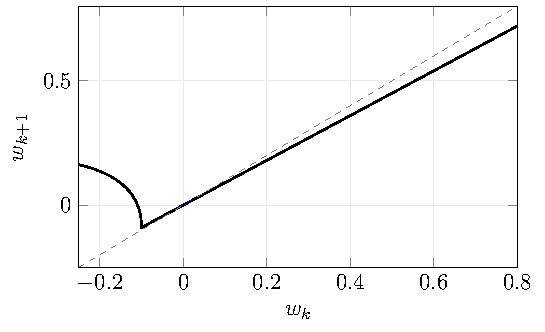
\includegraphics[width=1\linewidth]{graphics_v3/sr_m01.pdf}
         \caption{$\mu=-0.1$}
         \label{fig:s_m01}
     \end{subfigure}
     \begin{subfigure}[b]{0.48\linewidth}
         \centering
         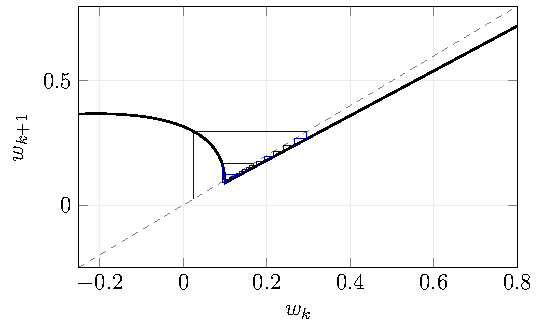
\includegraphics[width=1\linewidth]{graphics_v3/sr_01.pdf}
         \caption{$\mu=0.1$}
         \label{fig:s_01}
     \end{subfigure}
     \caption{Egy dimenziós square-root map különböző $\mu$ értékekre $\nu=0,9$ esetén}\label{fig:square-root}
\end{figure}

A \ref{fig:bif}. ábra rögzített $\nu$ mellett változó $\mu$-höz tartozó, tranziens utáni iterátumokat mutat. A különböző periódusú ablakok és a rendezetlen ponthalmazok a \emph{ciklusok periódusáról}, nem az egyensúlyi helyek számáról adnak információt. Kaotikusság megállapításához például pozitív legnagyobb Ljapunov-exponenst és numerikus konvergenciát is vizsgálni kell. A $\nu$ itt a leképezés sima ágának kontrakciós paramétere; nem azonos közvetlenül a mechanikai csillapítási tényezővel. A korábban megadott $1/4$ és $2/3$ határokat külön levezetés nélkül nem használjuk általános osztályozási tételként.

Az ábrák újraszámolhatók a \texttt{codes/square\_root\_figures\_v3.py} programmal. A bifurkációs mintavételben minden paraméterértéknél azonos kezdeti állapotból indulunk; több együtt létező attraktor teljes feltérképezéséhez több kezdeti állapot szükséges.

\begin{figure}[ht!]
\centering
\begin{subfigure}[b]{0.48\linewidth}
         \centering
         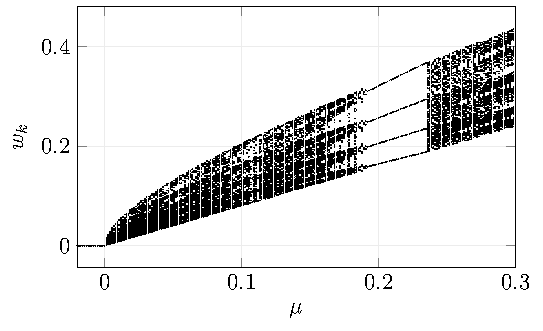
\includegraphics[width=1\linewidth]{graphics_v3/bif_08.pdf}
         \caption{$\nu=0.8$}
         \label{fig:kis_csillapitas}
     \end{subfigure}
     \begin{subfigure}[b]{0.48\linewidth}
         \centering
         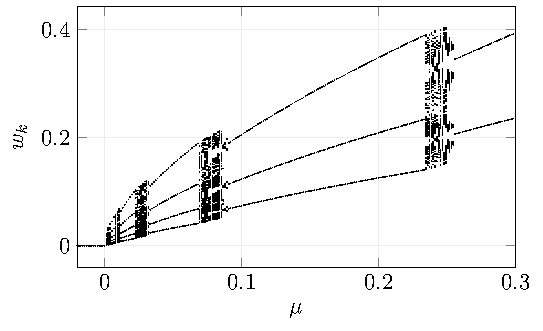
\includegraphics[width=1\linewidth]{graphics_v3/bif_06.pdf}
         \caption{$\nu=0.6$}
         \label{fig:kozepes_csillapitas}
     \end{subfigure}
     \begin{subfigure}[b]{0.48\linewidth}
         \centering
         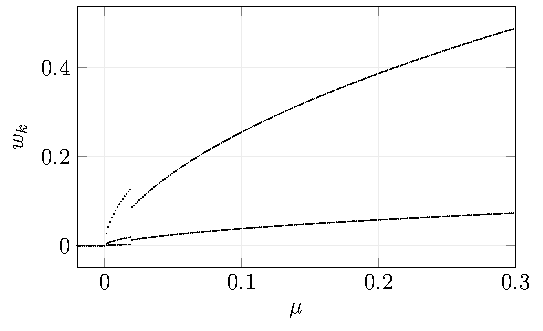
\includegraphics[width=1\linewidth]{graphics_v3/bif_015.pdf}
         \caption{$\nu=0.15$}
         \label{fig:nagy_csillapitas}
     \end{subfigure}
     \caption{Bifurkációs diagram az 1D square-root mapra vonatkozóan különböző $\nu$ értékek esetén (bifurkációs paraméter: $\mu$)}\label{fig:bif}
\end{figure}

\newpage
\exampleend

